\chapter{Common Aspects to Multi-b SUSY Searches}
\label{chap:multib_general}

The main results presented in this thesis are the two analyses described in Chapter \ref{chap:strong_prod} and Chapter \ref{chap:ewk_prod}. While these analyses target two different \gls{susy} models they have many commonalities, since they both target \gls{susy} models leading to final states rich in b-jets and \met. This Chapter highlights these common aspects: Section \ref{sec:simplified_models} describes the philosophy of simplified models, used to design the signal models, Section \ref{sec:common_backgrounds} focuses on the background sources from \gls{sm} processes and how they are modeled in the analyses. 
Section \ref{sec:common_obj_def} focuses on the definition of the physic objects, and Section \ref{sec:common_syst} introduces the main sources of 
systematic uncertainties.

\section{Simplified Models}
\label{sec:simplified_models}

Even with the simplifying assumptions of the \gls{pmssm}, discussed in Section \ref{sec:theory:pmssm}, a \gls{susy} model has to take into account a large number of free parameters, whose values can impact the characteristics of the particle production and decay. 
Simplified models \cite{Alves:2011wf} are very simple model of \gls{bsm} Physics involving only a few particles and decay mode, 
each one focusing on a specific signature, that can be used to optimize and interpret analyses targeting \gls{bsm} scenarios. 
In general simplified models can be viewed as a limit of more complete models, where all particles except a few are too heavy to be 
produced in the interactions. This leads to a drastic reduction of the number of parameters: a simplified model can be described just by the production cross-section and mass of the few particles considered. 
The \glspl{br} of the new particles can be a parameter of the simplified model as well, even if it is in general easier to consider each decay chain as a separate simplified model with 100\% \gls{br}.
When simplified models are used to discover or exclude a certain topology, it is important to connect the results obtained to more general models, 
which can be done for example relaxing the restrictions on the \gls{br} of the \gls{bsm} particles or allowing more particles to take part to the interaction.

\section{Analysis Strategy}

The analysis strategy is based on the definition of the \glspl{sr}, signal-enriched regions defined by selections on the relevant kinematic variables with the goal of maximizing the sensitivity to specific benchmark models. 
After the \glspl{sr} are defined, the central point of the analysis is an accurate estimate of the number of events expected from \gls{sm} processes (background events) in these regions, and of the associated uncertainty. 
With the background estimate in hand, it is possible to look at the observed yields in data and compare it with the expectations;
this comparison, performed with the statistical methods discussed in Chapter \ref{chap:stat}, allows to quantify the significance of an excess or to place limits on \gls{bsm} signal models.

The estimate of the expected background events can be performed with different techniques. In particular, in these thesis three types of techniques are used:
\begin{itemize}
\item A first option is to take the background estimate directly from \gls{mc} simulation. 
\item The \gls{mc} estimate can be improved by normalizing each process in a dedicated \gls{cr}, which is a region non overlapping with the \gls{sr} but kinematically close to it, enriched in the background process that we want to normalize and with a very low expected signal fraction. Since \gls{cr} and \gls{sr} must be non-overlapping, some of the selection of the \gls{sr} are inverted to design the \gls{cr}; the extrapolation of the background normalization factor form the \gls{cr} to the \gls{sr} is tested in dedicated \glspl{vr}. Figure \ref{fig:susy_common:CRschema} shows a schematic view of the relation between \glspl{cr}, \glspl{vr} and \glspl{vr}. A simplified example of how the usage of \glspl{cr} can improve the analysis also from the point of view of systematic uncertainties is discussed in Section \ref{sec:example_cr}. 
\item In some cases, a background estimate that relies only on data and not on \gls{mc} simulation is preferred. In these cases we speak of data-driven background estimate.
\end{itemize}

\begin{figure}
\centering
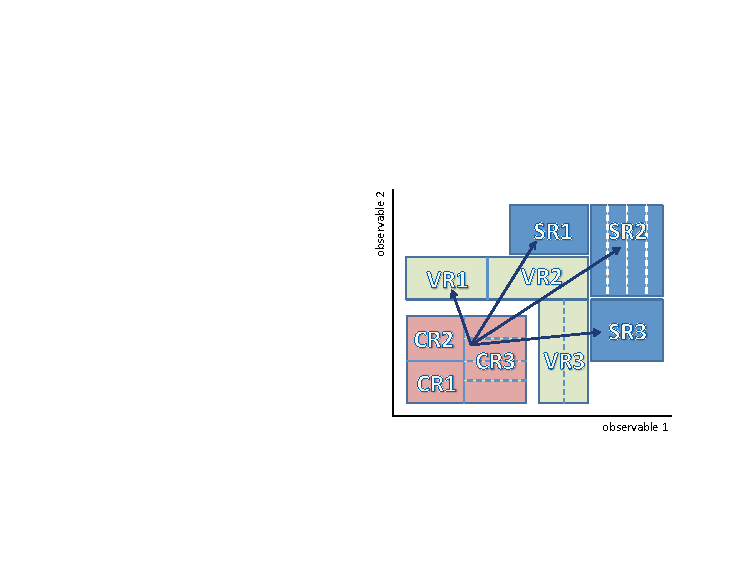
\includegraphics[width=0.55\textwidth]{figures/susy_common/CR_VR}
\caption{Schematic view of the relation between \glspl{cr}, \glspl{vr} and \glspl{vr}. Figure from Ref. \cite{Baak:2014wma}.}
\label{fig:susy_common:CRschema}
\end{figure}
 
In each of the analyses described in the next two chapters, two different analysis strategies are carried out in parallel:
\begin{description}
\item[Cut-and-count] Several \glspl{sr} are designed, each optimized to maximize the discovery significance to a specific region of the phase space, represented by one benchmark model. Cut-and-count \glspl{sr} are useful also to provide simple and powerful model-independent \glspl{ul}, that are easy to re-interpret for signal models different than the ones considered in the analysis. 

\item[Multi-bin] In this case, the \glspl{sr} are non-overlapping. This requirement conflicts with the simple choice of the best selection to maximize the significance, which means that the individual discovery power of each \gls{sr} is smaller than in the case of cut-and-count \glspl{sr}. On the other hand, having non-overlapping \glspl{sr} allows to statistically combine them in the Likelihood fit, leading to a stronger model-dependent expected \gls{ul}. The increase in expected exclusion obtained with the combination of several regions is shown in Section \ref{sec:example_combi}.
 
\end{description}



\section{Background Processes and their modelling}
\label{sec:common_backgrounds}

This section describes the main background processes from the \gls{sm} in the analysis regions and the way they are 
modeled in the analyses discussed in the next two chapters. In general, the modelling is based on \gls{mc} simulations for
all the backgrounds, except multi-jet which is emulated with a data-driven technique.
For the main background, pair production of top quark pairs (\ttbar), the shape of the different distributions is obtained from \gls{mc}
but the normalization is data-driven, derived in specifically designed \gls{cr} as described in Section \ref{sec:analyses:cr}.


\subsection{Top quark pair production}

Given the presence of several b-jets in the final state, \ttbar production in association with jets constitutes the main source of \gls{sm} background in all the analysis regions. \ttbar production is mediated by the strong interaction, and it can occur through quark-antiquark annihilation (Fig. \ref{fig:ttbar_prod_qq}) or through gluon-gluon fusion (Fig. \ref{fig:ttbar_prod_gg_1} to \ref{fig:ttbar_prod_gg_3}). When the \gls{lhc} is running at 13 TeV, the threshold fraction of the proton energy that must be carried by each parton in order to have sufficient energy to produce a system of two top quarks 
is about 2.6\%. At these low fractions, the \gls{partdf} of the gluon is higher than the \gls{partdf} of quarks and much higher than the \gls{pdf} of the antiquarks, so gluon-gluon fusion is the dominant \ttbar production mode at the \gls{lhc}.

\begin{figure}[h]
\centering 
\subfigure[]{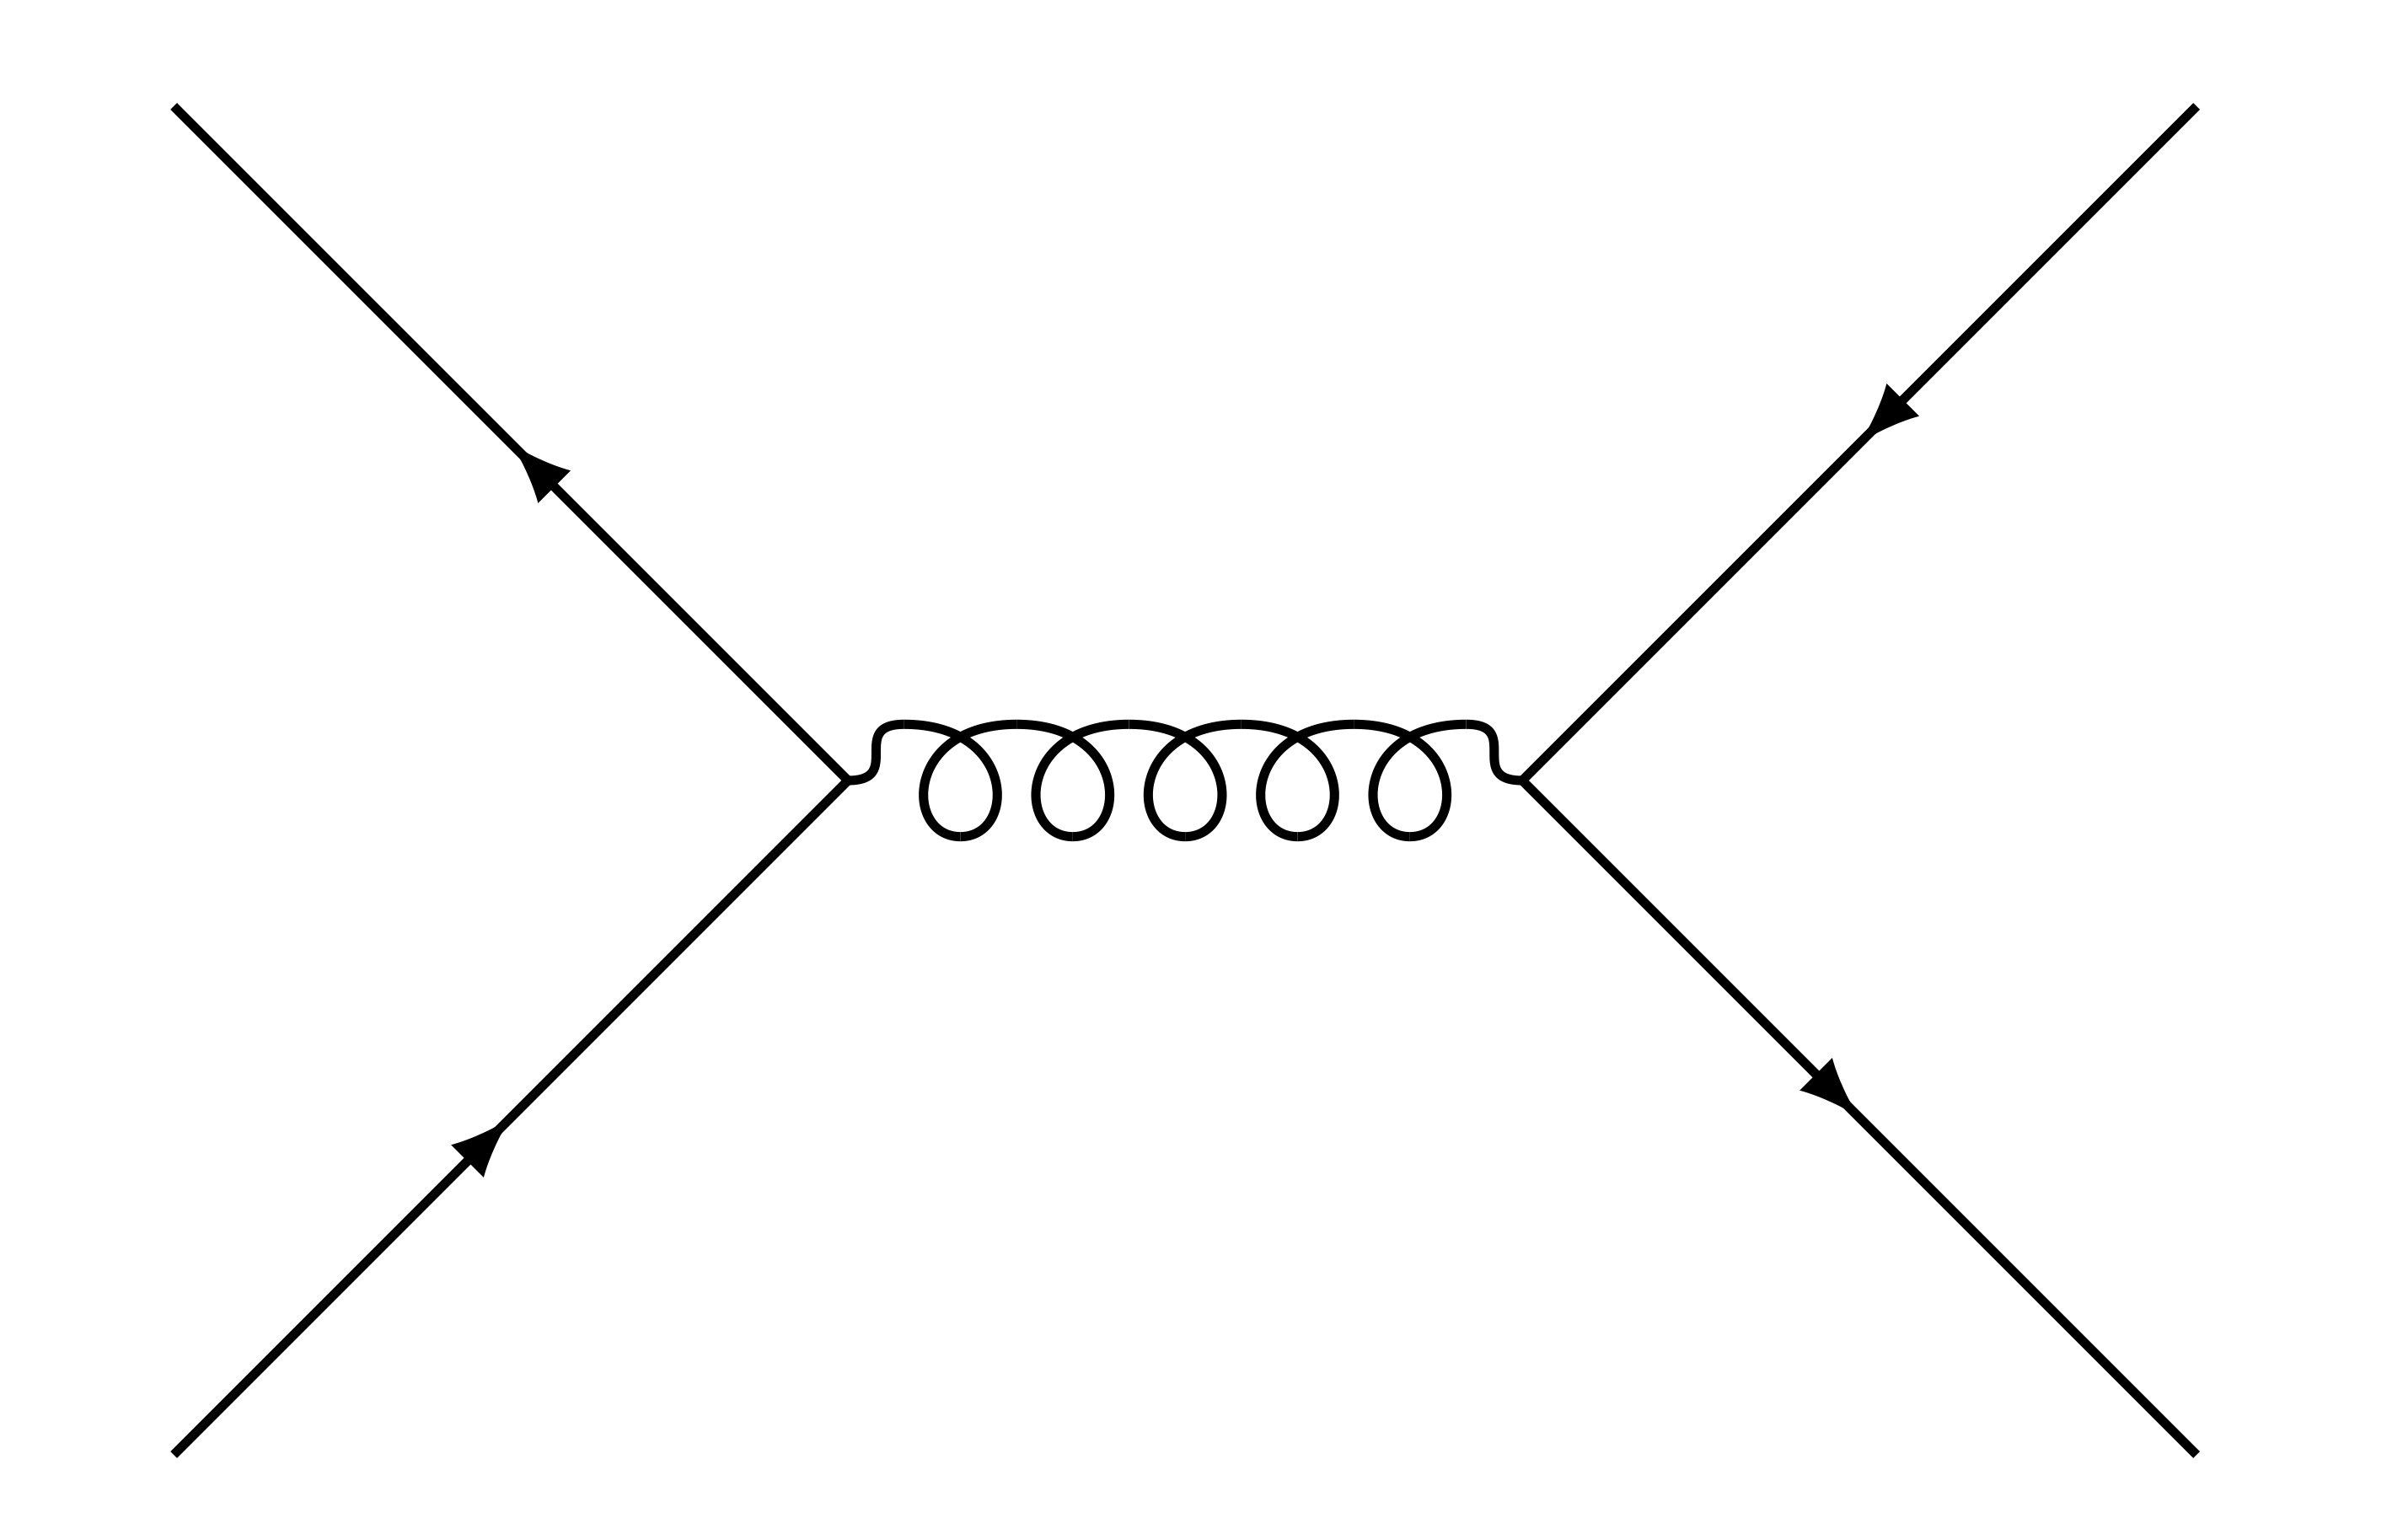
\includegraphics[width=0.3\textwidth]{figures/susy_common/feynman/ttbar_4}\label{fig:ttbar_prod_qq}}\\
\subfigure[]{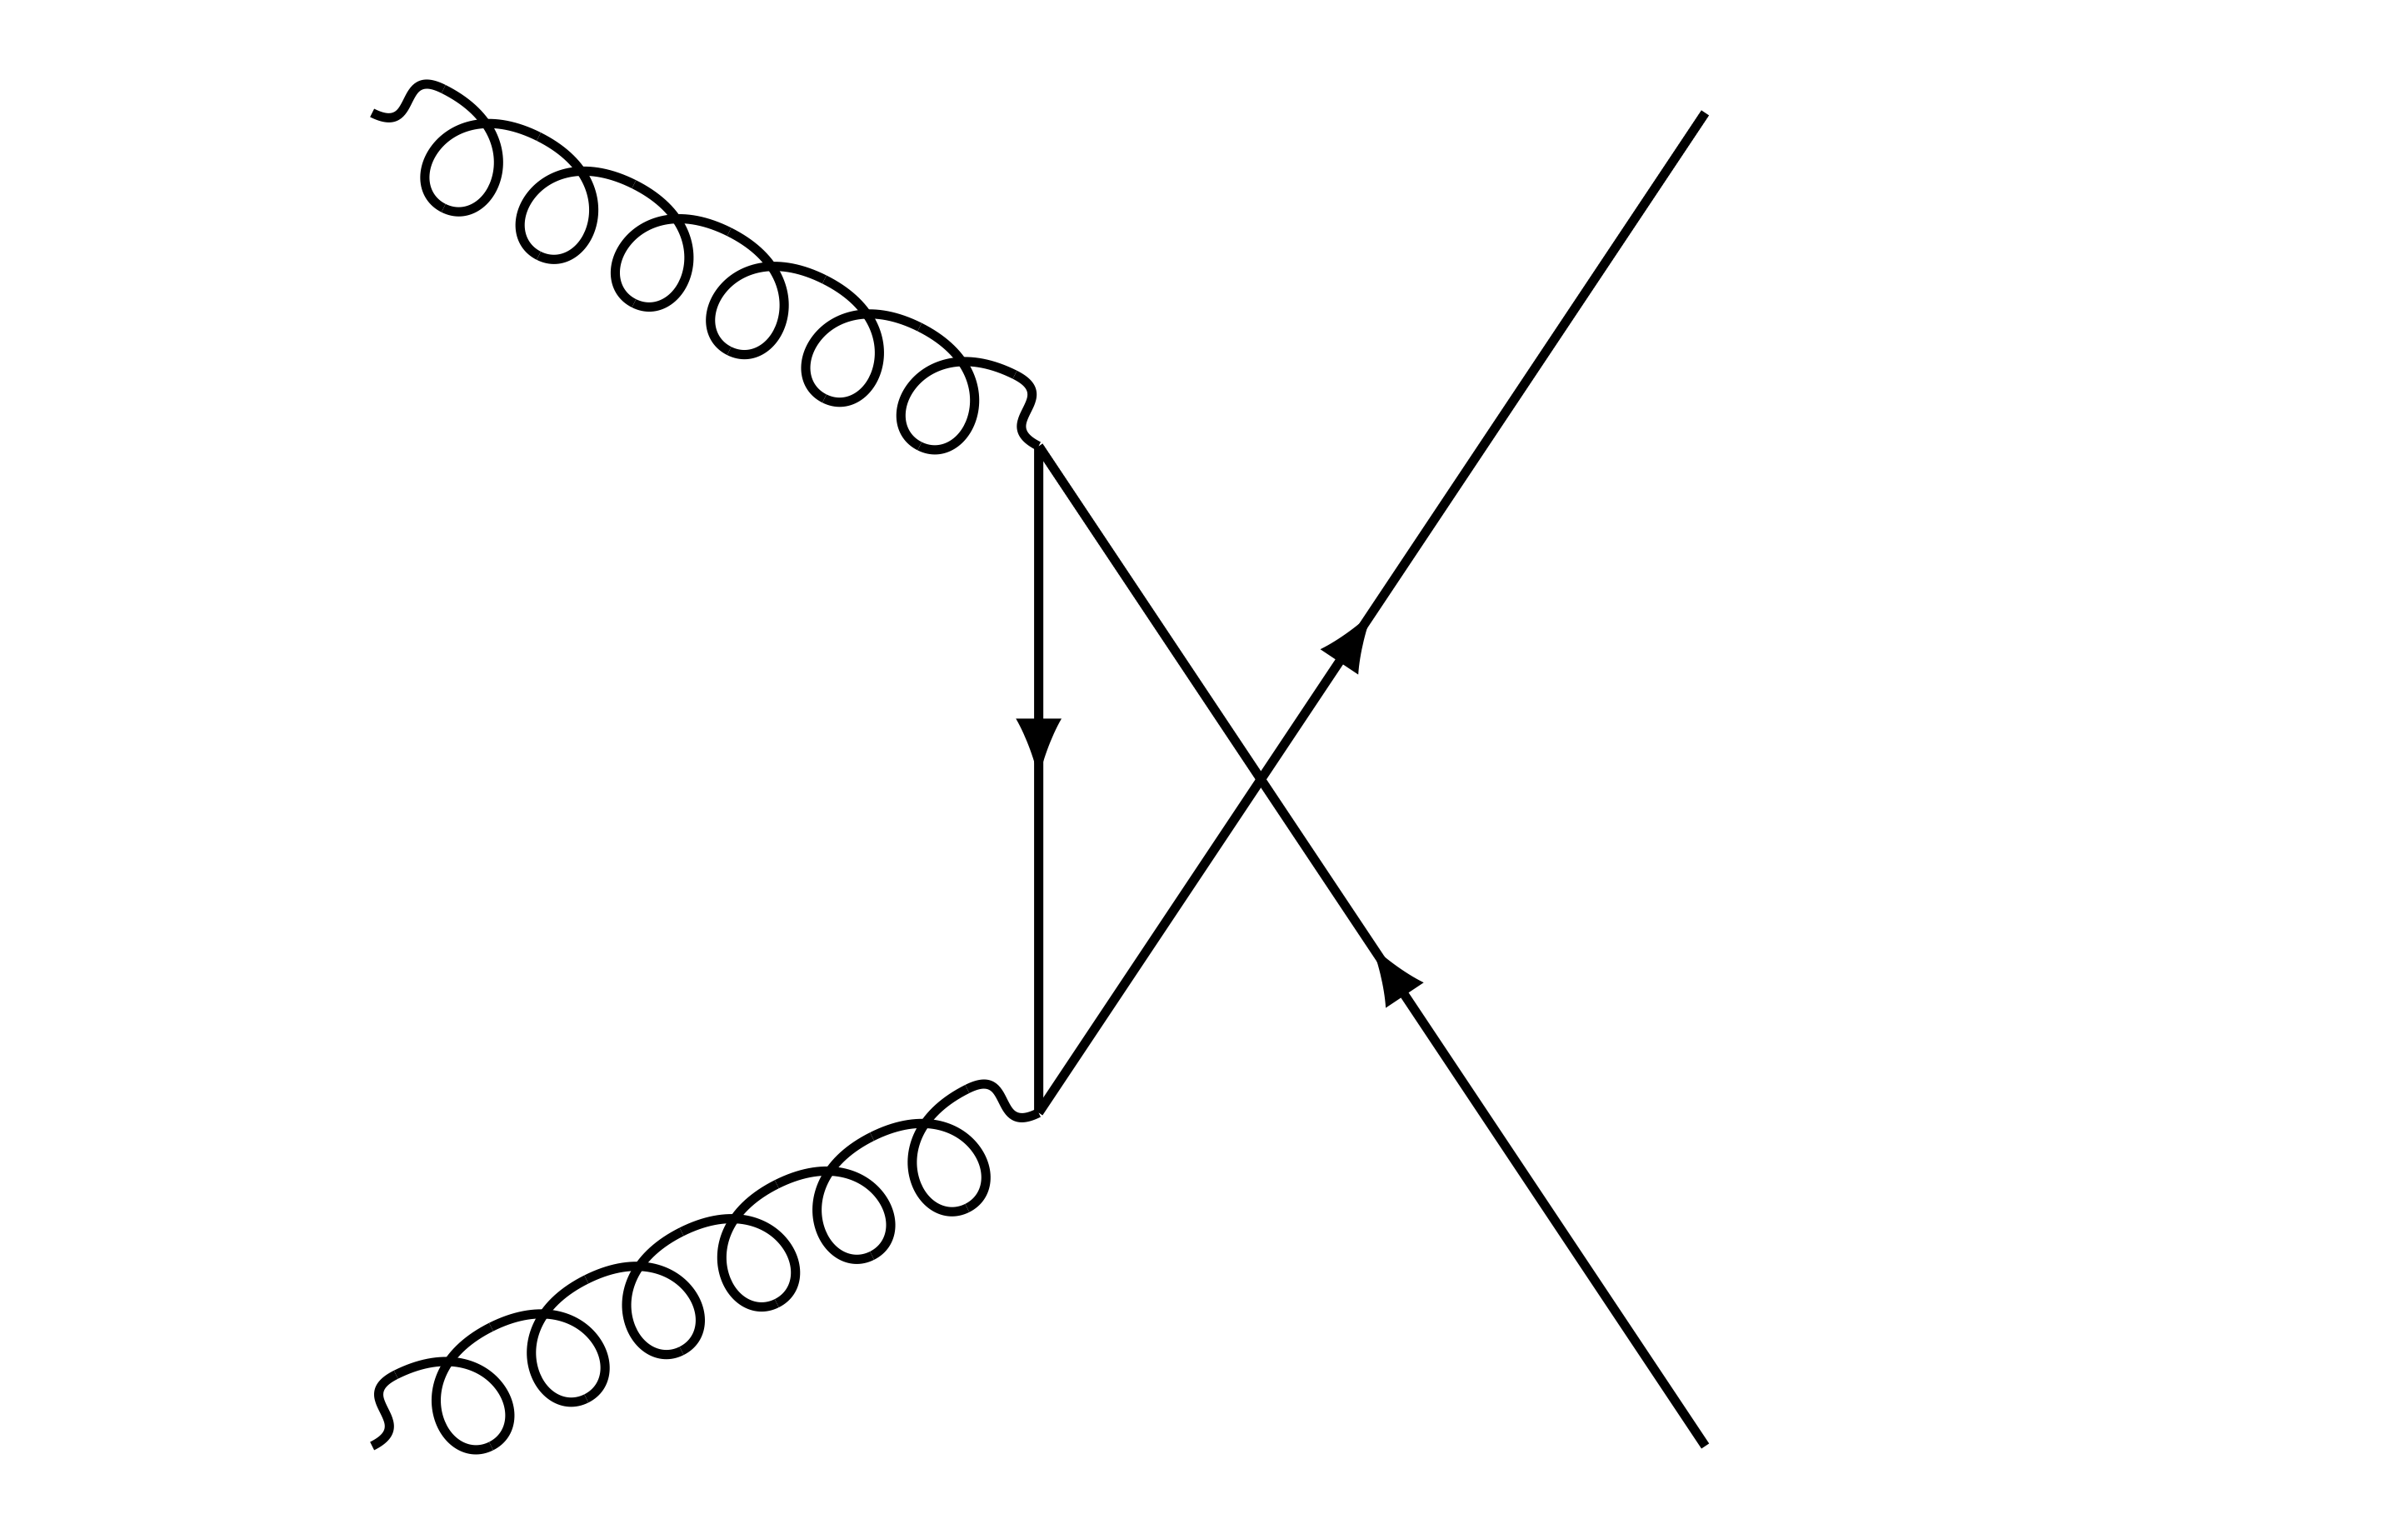
\includegraphics[width=0.3\textwidth]{figures/susy_common/feynman/ttbar_1}\label{fig:ttbar_prod_gg_1}}
\subfigure[]{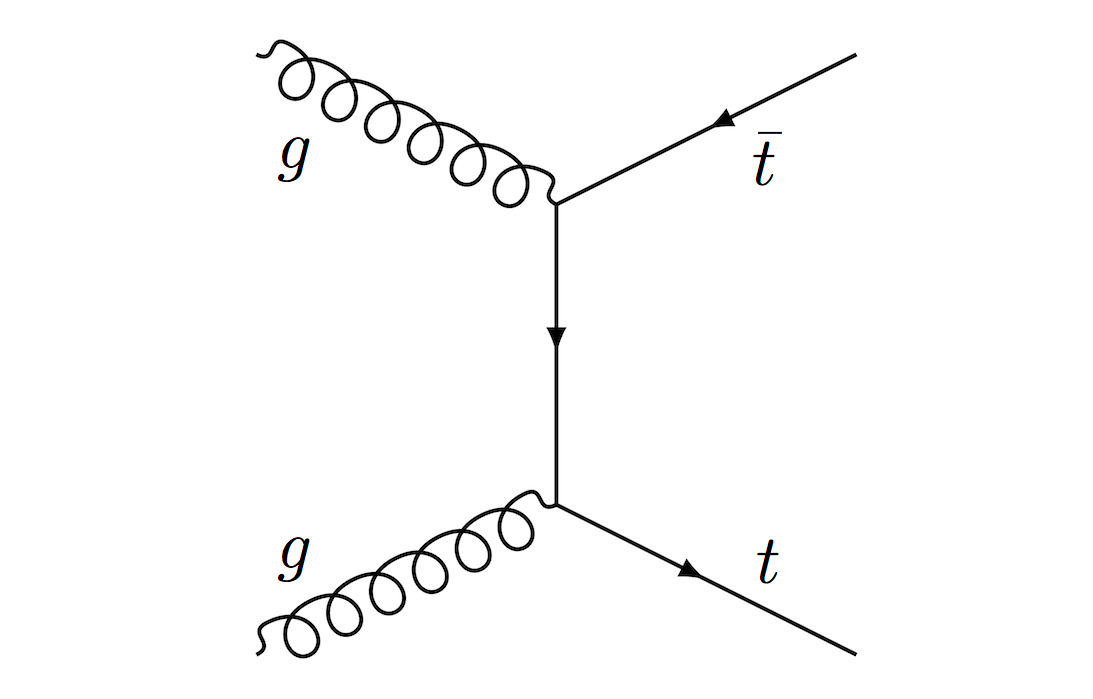
\includegraphics[width=0.3\textwidth]{figures/susy_common/feynman/ttbar_3}\label{fig:ttbar_prod_gg_2}}
\subfigure[]{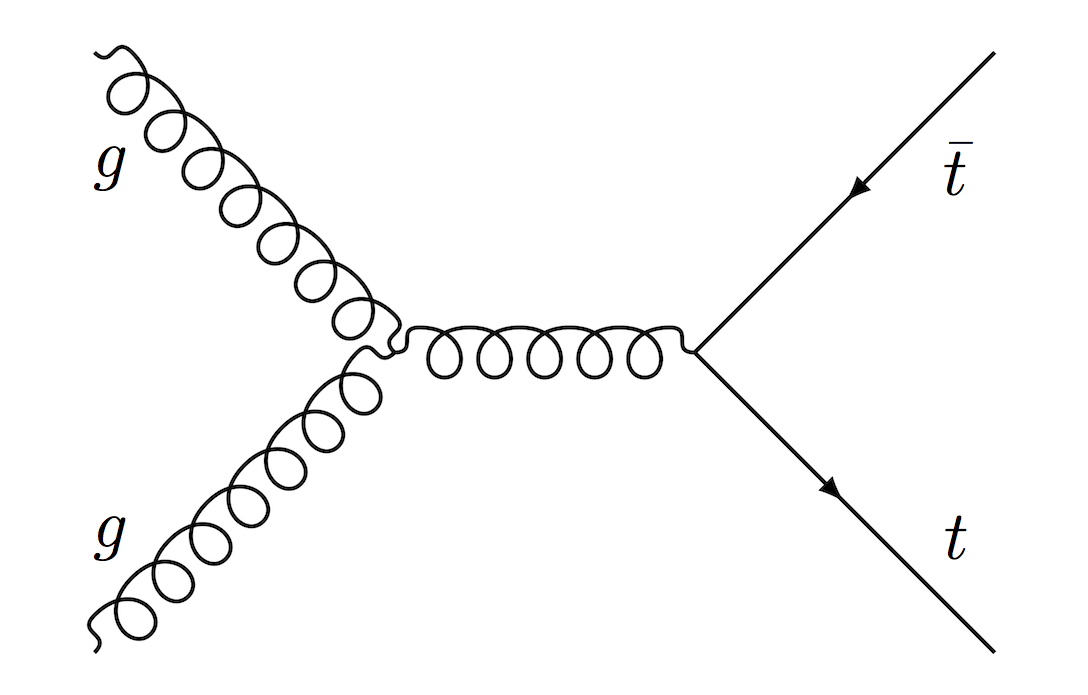
\includegraphics[width=0.3\textwidth]{figures/susy_common/feynman/ttbar_2}\label{fig:ttbar_prod_gg_3}}
\caption{\gls{lo} Feynman diagram for the production of top quark pairs initiated by \subref{fig:ttbar_prod_qq} quark-antiquark annihilation and \subref{fig:ttbar_prod_gg_1}-\subref{fig:ttbar_prod_gg_3} gluon-gluon fusion.}\label{fig:ttbar_prod}
\end{figure}

\subsubsection{Truth-level classification: \ttbar decays}

\subsubsection{Truth-level classification: flavour of the associated jets}

\subsection{Control Regions}
\label{sec:analyses:cr}

\subsection{Single top quark production}

While the production of a \ttbar pair is mediated by strong interaction, in the case of a single top quark the production occurs through electroweak 
couplings. There are three possible production channels, illustrated in Fig. \ref{fig:single_top_prod}: the Wt-channel, where a top quark and a W boson are produced, the t-channel, and the s-channel. 

\subsection{Vector boson}

\subsection{Multi-bonson}

\subsection{\ttbar + V production}

\subsection{Multi-jet}


\section{Object Definition}
\label{sec:common_obj_def}

\section{Systematic Uncertainties}
\label{sec:common_syst}

\subsection{Experimental Systematic Uncertainties}

\subsection{Modeling Uncertainties} 

